\chapter{Introduction}

\section{Motivation}
\gls{ic} is a faculty of \gls{kmitl}. 
\gls{ic} has been up and running well for 6 years.
About 25 employees are working here.
Their main objective is to provide educational services to students. 
Currently, they are having three major problems involved with their accumulating documents.
First, the organization takes countless hours to store and retrieve documents even though they have organized documents into categories.
Simply retrieving a document can take hours or even weeks. 
This problem hinders employee's productivity when they need to retrieve many documents. 

Second problem is losing track of document during its workflow execution. 
A workflow is a series of repeatable steps performed in a sequential manner to reach a goal.
For instance, Mr.A wants video \enquote*{X} hosted on a website \enquote*{Y} to be taken down due to copyright violation.
He has to go through Y's copyright claim workflow to satisfy his goal.
First, Mr.A have to report the claim to Y.
Y's administrator evaluates the claim.
If the claim is valid, administrator takes down X.
This task marks the end of Y's workflow that Mr.A has to go through.
The workflow provides specification, execution and control of business processes \cite{Jablonski:1996:WMM}. 
A person who hold responsibility of a document will execute actions based on their assigned roles.

Third problem is that some \gls{ic}'s workflows are so complicated that they are difficult to keep track of.
There are many actions and conditions to execute.
Many people from both inside and outside of the organization may involve during workflow's execution.
Supplementary documents, or so called attachments, may need to be attached with original document in order to pass some certain guidelines.
As a result, \gls{ic} can't certainly identify who is currently involved and what actions they must do with that document.
They can't track attachments effectively causing delay in archiving.

Our proposed solution is to manage, store, and retrieve documents digitally using a computer software.
The employee will use less time to search and be less error-prone.
We will create a system that provide ability to search and to track documents.
We are working on \MakeLowercase{\projTitle} for \gls{ic}, \kmitl, or so called Monkey Office.
Because we want to provide a system to manage documents within \gls{ic}.
Once we succeed, \gls{ic} can manage and track documents effectively, thus, increase organization's productivity.

\section{Objective}
% list of our primary objectives
Our primary objectives are
\begin{enumerate}
\item To design \gls{ic}'s workflow model associated with each type of documents.\footnote{
	Although workflow is not our main focus, we work closely with other researchers on \enquote{web-based automatic form generated system} \cite{web-based-form}.
	Not only we share a similar objective, but also we have to link our system with them.
	We need their general workflow models to achieve this objective.
	}
\item To track and to report the current task during workflow's execution.
\item To store and retrieve digital documents corresponding to outgoing or finished workflows from and to \gls{ic}'s server.
\end{enumerate}

\section{Scope}
We are going to develop a web-based application hosted on an \gls{ic}'s server.
Only people within \gls{ic} and granted external users can access the system.
To be specific, there are four types of users.
\begin{enumerate}
\item \gls{ic}'s administrative staffs.
\item \gls{kmitl} lecturers who is assigned to \gls{ic}.
\item Students who are currently enrolled in \gls{ic}.
\item External users who is allowed to access the system by \gls{ic} e.g.\ alumni students.
\end{enumerate}

We would like to clarify these two words---workflow and document---in terms of our project. %transition
% Explain what is a workflow
A \enquote{workflow} is a collection of repeatable tasks performed to achieve a goal \cite{Jablonski:1996:WMM}.
It can execute multiple tasks sequentially or simultaneously depending on how it is created.
For instance, there are four tasks namely \enquote*{P}, \enquote*{Q}, \enquote*{R}, and \enquote*{S}.
The workflow executes P first followed by Q.
Then, it executes R and S at the same time.
The execution of P and Q are sequential because Q have wait for P to finish first.
On the other hand, the execution of R and S are simultaneous because R and S execute in parallel.
In organizations, the goal of the document is get them approved, distributed, or archived.
Each task may perform with specific conditions.
A person, machine, group of persons or machines are responsible to carry out the task \cite{wfMangement}. 
% Explain what is a document
A \enquote{document} is a computer's executable file associates with each user's workflow.
For example, a user executes workflow \enquote*{X}.
One of the X's task requires user to upload a \gls{pdf} file as an input.
The task will produce a reply letter as an output.
There are two documents in X---the \gls{pdf} report and the reply letter.
% Explain how workflow and document are related
So, how workflow and document are related together?
A document can be an input or end-product of the task.
The task may require a certain document to execute.
Other documents may be produced by the task.

Our primary focus is digital documents produced from tasks in the workflow.
The system has to manage workflows which are created officially by \gls{ic} and documents produced by tasks.
The system offer document file hosting services to users for reusing them later.
Hosted documents that are not used by the workflow is not in the scope of this project.
Uploaded documents that is not in the system's file hosting service is in the scope if \gls{ic} requires them in one of the task in workflow.
This thesis conducts only on the following two types of documents.
% How these 7 types are related to form, resulting docs, attachments, ...
\begin{enumerate}
\item Electronic form \hfill \\
A formatted document with blank fields that prompts user to fill in.
Forms are created according to \gls{ic}'s work procedure and instruction.
Work procedure provides details on working procedures, departments, or persons who hold responsibilities for documents.
Work instruction indicates employee's roles and responsibilities.
\gls{ic} defines non-filled form as \enquote*{Form} and already filled form as \enquote*{Record}.
By the time of writing, this project conduct with three sub-types forms.
\begin{enumerate}
\item Absence form \hfill \\
For \gls{ic}'s employee and students to take days off due to personal or business reasons.
\item Student internship form \hfill \\
For \gls{ic} students who is above Year 2 to gain work experience in software industry during a summer semester.
\item Conference outside \gls{kmitl} form \hfill \\
For lecturers to request going to a conference outside \gls{kmitl}.
\end{enumerate}
Because all of these forms are in paper-based format, we have to convert them into the electronic form.
Meaning that a system displays the form on a computer screen waiting for a user to fill in required blank fields.
\item External document \hfill \\
Documents received from other individuals or departments in order to proceed some tasks in a workflow.
If received document is in paper form, it has to be scanned by a scanner first.
The task includes these documents as attachments.
\end{enumerate}

\section{Project plan}
The project starts at August 18th, 2015.
We expect to deliver it on March 25th, 2016.
For our project planing, we divide our work into 4 phases.
\begin{enumerate}
\item Plan and research (18/08/15 -- 30/10/15) \hfill \\
The first phase was to gather user's requirements by interviewing.
We interviewed with \gls{ic}'s vice dean because he is a client who came up with this project.
Then, we moved on to interviewing \gls{ic}'s employees asking about document related problem they encountered.
Next, we discussed about software tools that solve the problem.
\item Design and architecture (29/09/15 -- 23/11/15) \hfill \\
On the second phase, we designed the software architecture.
The architecture is the core of how software must behave, also to get an overview of system interaction.
Then, we designed a \gls{gui} of this system.
\item System implementation (7/12/15 -- 22/02/16) \hfill \\
This phase began writing source codes based on user requirements, designed architecture, and technical specification.
Later on, we connected each system's components together.
\item Testing (19/02/16 -- 07/03/16) \hfill \\
This phase ensured that systems ran correctly with user and system requirements.
We also conducted user acceptance testing.
Then, We evaluated testing result.
If the result were satisfying, we would deploy the system to \gls{ic}'s server.
\end{enumerate}

\begin{landscape}
\begin{figure}
\centering
\caption{Project's schedule shown as Gantt chart}
\label{fig:project-schedule}
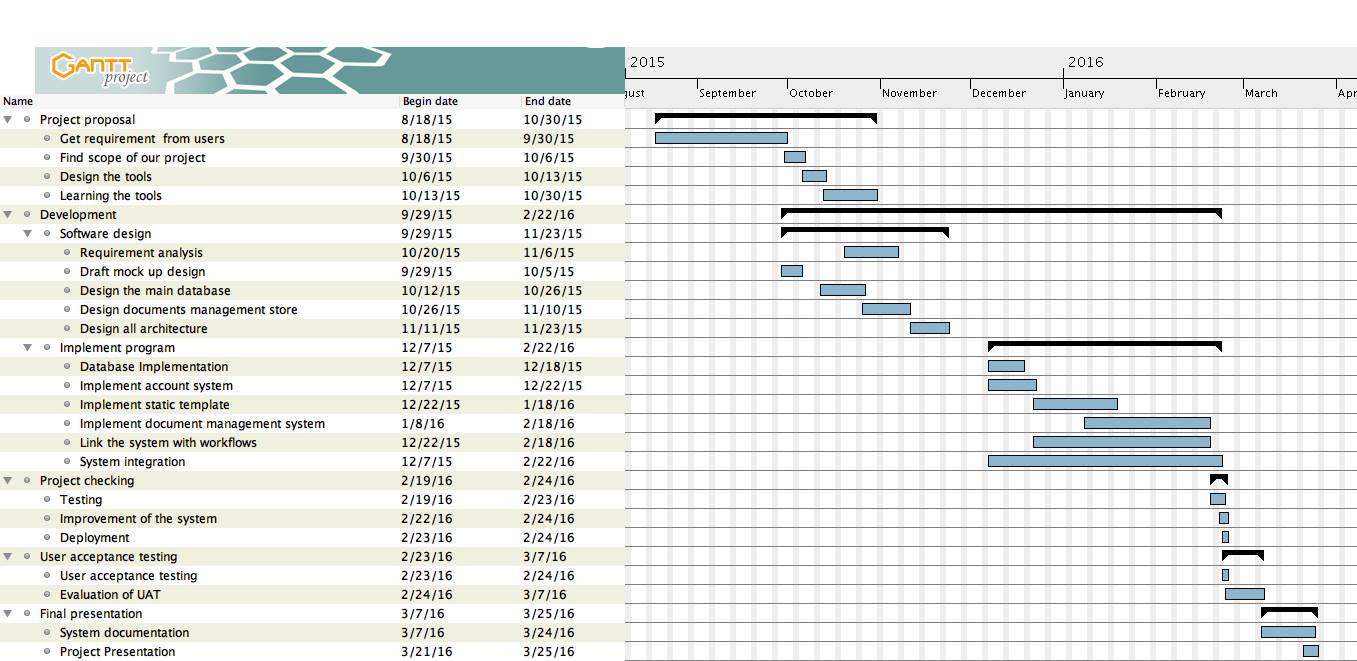
\includegraphics[scale=0.4]{res/project_plan}
\end{figure}
\end{landscape}